\section{Z80emu{\dywiz}core}

\emph{Z80emu{\dywiz}core} to główny moduł odpowiedzialny za emulację. Korzysta on z biblioteki \emph{XBit}. Rysunek nr \ref{img:z80EmuPackage} prezentuje podział kodu modułu na następujące pakiety (nazwy pakietów zostały skrócone~o prefiks "org.tomaszkowalczyk94.z80emu.core." aby były bardziej czytelne):

\begin{itemize}  
    \item \emph{helper} - zawiera klasy wspomagające wykonywanie powtarzalnych operacji,
    \item \emph{instruction} - pakiet grupujący klasy implementujące rozkazy procesora; zawiera kolejne zagnieżdżone paczki mające za zadanie grupować instrukcje w kategorie np. rozkazy skoku,
    \item \emph{io} - pliki odpowiedzialne za implementację symulatorów urządzeń wejścia/wyjścia podłączonych do wirtualnego CPU,
    \item \emph{memory} - klasy definiujące reprezentacje pamięci procesora,
    \item \emph{register} - klasy odpowiedzialne za rejestry CPU.
\end{itemize}


\begin{figure}[h]
		\centering
		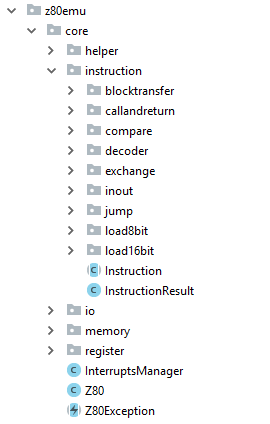
\includegraphics[width=0.4\textwidth]{z80EmuPackage}
		\caption{Podział na pakiety projektu Z80emu-core}
		\label{img:z80EmuPackage}
\end{figure}

\subsection{Metoda runOneInstruction() klasy Z80}
Najważniejszą metodą w module jest \emph{runOneInstruction()}, zaprezentowana w listingu \ref{listing:runOneInstruction}. Pobiera ona kolejną instrukcję CPU do wykonania z pamięci (linia nr 4), następnie wykonuje ten rozkaz (linie nr 6-9) i aktualizuje liczniki (linie nr 11-16). Ważnym elementem tego podprogramu jest linia nr 1,  wywołująca metodę \emph{handleInterrupts()}, której zadaniem jest obsłużyć ewentualne przerwanie.

\begin{listing}[h]
	\inputminted{java}{listings/z80emu-core/runOneInstruction.java}
	\caption{Metoda runOneInstruction()}
	\label{listing:runOneInstruction}
\end{listing}

\subsection{Dekodowanie instrukcji}
Zilog Z80 jest procesorem, który używa rozkazów o różnej długości \mbox{(od 1 bajtu do 4)}. W~związku z~tym implementacja metody dekodującej instrukcje jest złożona. Nie jest możliwe przesłanie do niej jako parametr ciągu bajtów do interpretacji, ponieważ nieznana jest jego docelowa długość. Jedną z opcji byłoby nadmiarowe przesłanie zawsze czterech bajtów, ponieważ taka może być maksymalna długość rozkazu w emulowanym procesorze. Uznano jednak, że lepszym rozwiązaniem będzie przekazanie klasie dekodującej, obiektu reprezentującego pamięć. Dzięki takiemu rozwiązaniu jest możliwe odczytanie dowolnego bajtu pamięci przez klasę dekodującą.
Zmniejszy to częstotliwość wywoływania metod odczytu pamięci w newralgicznej części emulatora. 

W listingu \ref{listing:decodeInstruction} zaprezentowano fragment kodu odpowiedzialnego za dekodowanie rozkazu. Metoda \emph{decode} przyjmuje dwa parametry:obiekt reprezentujący pamięć oraz wartość rejestru \emph{PC}. W liniach 3-5 zamieszczone zostało dekodowanie zawartości pamięci zawierającej początkowy bajt rozkazu, który przekazano do instrukcji \emph{switch}. Jeśli jest możliwa interpretacja rozkazu na podstawie pierwszego bajtu, zostaje zwrócony obiekt reprezentujący go tak jak w linii nr 12 lub 14. W przypadku gdy pierwszy bajt jest niewystarczający, interpretacja rozkazu zostaje oddelegowana do oddzielnych metod, które pobierają kolejną komórkę pamięci tak jak w linii nr 9.  

\begin{listing}[h]
	\inputminted{java}{listings/z80emu-core/decodeInstruction.java}
	\caption{Dekodowanie rozkazu procesora}
	\label{listing:decodeInstruction}
\end{listing}

\subsection{Implementacja przykładowej instrukcji}
Każdy rozkaz procesora jest reprezentowany jako osobna klasa. Przykład takiej klasy przedstawiono w listingu \ref{listing:exampleInstruction}. Wykonuje ona instrukcje \emph{LD A, (BC)}, która ma za zadanie wczytać do rejestru \emph{A} wartość komórki pamięci o~adresie przechowywanym w rejestrze \emph{BC} (linie 9-15). Po wykonaniu tej operacji, metoda \emph{execute} zwraca obiekt \mbox{\emph{InstructionResult}} (linia~17), który zawiera informacje o przebiegu wykonania instrukcji, takie jak:

\begin{itemize}  
    \item liczba cykli maszynowych,
    \item liczba taktów zegara,
    \item czas wykonania w milisekundach,
    \item rozmiar rozkazu w bajtach (aby poprawnie zwiększyć wartość rejestru \emph{PC}).
\end{itemize}

\begin{listing}[h]
	\inputminted{java}{listings/z80emu-core/exampleInstruction.java}
	\caption{Fragment kodu odpowiedzialnego za dekodowanie rozkazu procesora}
	\label{listing:exampleInstruction}
\end{listing}

\subsection{Przerwania}
Zilog Z80 jest procesorem realizującym dwa rodzaje przerwań:
\begin{itemize}  
    \item przerwanie niemaskowalne - przerwanie, które nie może zostać wyłączone przez programistę. Wywoływane jest przez podanie sygnału na fizyczne wejście procesora NMI (ang. \emph{non-maskable interrupt}). Po przyjęciu przerwania, procesor wykonuje restart do adresu \emph{0066h},
    \item przerwanie maskowalne - wywoływane poprzez fizyczny sygnał INT (ang. \emph{interrupt}). Procesor może zareagować na nie na trzy sposoby:
    \begin{itemize}
        \item tryb 0 - urządzenie przerywające umieszcza na magistrali danych instrukcje do wykonania. Ponieważ szyna danych jest 8-bitowa, rozkaz umieszczony na niej musi być jednobajtowy. Najczęściej jest to instrukcja restartu \cite{manual},
        \item tryb 1 - wykonuje restart do adresu \emph{0038h},
        \item tryb 2 - procesor wykonuje skok do adresu, którego starszy bajt jest umieszczony w rejestrze \empty{I}, a młodszy dostarcza urządzenie przerywające,
    \end{itemize}
    Tryby może przełączać programista, używając instrukcji \emph{IM 0}, \emph{IM 1} i \emph{IM 2}.
\end{itemize}

\subsubsection{Przerwanie niemaskowalne}
Obsługa przerwania niemaskowalnego polega na umieszczeniu na szczycie stosu aktualnej wartości rejestru \emph{PC}. Następnie do licznika rozkazów zapisano wartość \emph{0066h}. Fragment kodu realizujący te operacje umieszczono w metodzie \emph{handleNmiInterrupt} zaprezentowanej w listingu \ref{listing:handleNmiInterrupt}

\begin{listing}[h]
	\inputminted{java}{listings/z80emu-core/handleNmiInterrupt.java}
	\caption{Metoda obsługująca przerwanie niemaskowalne}
	\label{listing:handleNmiInterrupt}
\end{listing}

\subsubsection{Przerwanie maskowalne}
Implementacja obsługi przerwania maskowalnego pokazana na listingu \ref{listing:handleInterrupt}, w~związku z~koniecznością uwzględnienia trzech sposobów reagowania na nie, jest bardziej złożona. W pierwszej kolejności odkładana jest wartość rejestru \emph{PC} na stos (linia nr 3). Następnie sprawdzany zostaje aktywny tryb przerwania (linia nr 5), przechowywany w polu typu wyliczeniowego \emph{interruptionMode}. W dalszej części program ulega rozgałęzieniu zależnie od aktywnego trybu przerwania:
\begin{itemize}  
    \item dla trybu nr 0 - dekodowana jest jedno-bajtowa instrukcja umieszczona na szynie danych, i wykonana (linie 7, 8),
    \item dla trybu nr 1 - podobnie jak w przerwaniu niemaskowalnym, wystarczy zmienić wartość rejestru \emph{PC}, w tym przypadki na \emph{0038h},
    \item dla trybu nr 2 - wartość rejestru \emph{PC} zostaje zmodyfikowana. Starszym bajtem jest rejestr \emph{I}, a młodszy to wartość przesłana przez urządzenie na szynę danych (linie 15 i 16. Nowa wartość rejestru \emph{PC} powinna być parzysta, z tego powodu zmieniono najmniej znaczący bit na \emph{0}.
\end{itemize}


\begin{listing}[h]
	\inputminted{java}{listings/z80emu-core/handleInterrupt.java}
	\caption{Metoda obsługująca przerwanie maskowalne}
	\label{listing:handleInterrupt}
\end{listing}

